This chapter introduces and explains the fundamentals to understand the rest of the this disseration. Related work is also reviewed and directly compared against the proposed project.

\section{Fundamentals on \acl*{SLAM} (\acs*{SLAM})}

From the beginning of civilization, mapping the surroundings has been a key concept for navigating the environment. In essence we faced the same problem as our ancestors: How do we map the environment and know our location within it? \acs*{SLAM} is the challenge of mapping the local environment of a moving entity (e.g. robot) and updating the map continuously as the entity moves through space. This is a massive problem to tackle on and of extreme importance to achieve full robot autonomy. A robot's autonomy is based on its understanding of its surrounding environment, which can be obtained through sensors. There are many types of sensors that are useful for this purpose, sensors such as:
\begin{itemize}
    \item \textbf{\acs*{LiDAR}s} cameras project infrared light into the environment and track the time it takes for the reflected light to return. By doing so, it is possible to calculate the distance between the camera and other objects. \acs*{LiDAR} has shrunk in size over the past decade and the cost was also dramatically reduced, making portable solutions possible.
    \item \textbf{RGB-D} cameras add depth information to the RGB channels used in standard cameras, creating what is known as a 3D PointCloud. Although it also uses infrared light to compute depth information, it works differently than a \acs*{LiDAR}. Depth is calculated by projecting a grid of infrared points onto the environment; the farther away an object it, the wider the gap between the points is.
    \item \textbf{\acs*{IMU}} transforms the information of accelerometer, gyroscope, and magnetometer sensors into accurate pose data. The gyroscope provides information about the rotation and the accelerometer provides information on linear velocity and angular acceleration. Magnenometers are not included in every \acs*{IMU}, but those that do can also provide direction relative to the magnetic north.
    \item \textbf{\acs*{GPS}} is a satellite-based navigation system that provides the latitude, longitude and altitude of an object on Earth.
\end{itemize}

Gather sensory information on the outside world is the first step, now \acs*{SLAM} could technically be split into two main problems, one that is mapping and the other localization. Although it is possible to know the localization without knowledge of the map, there will always be some localization information needed when mapping an environment, unless the entity has a fixed position.

\subsection{Localization}
Localization can take two forms: global or relative. 
Global localization gives the position in a global reference (for instance the Earth). Information provided by global localization can be viewed independently of other positions. It is generally given by \acs*{GPS} in the form of longitude, latitude and altitude.
Relative localization, as the name suggests, the current pose (position and orientation) is related to other pose. A pose's current state is usually determined by its last state. To compute relative localization it is common to use data from motion sensors, such as wheel encoders and \acs*{IMU}s, to estimate change in pose over time.
The procedure of estimating a change in pose over time by using sensory information is called odometry. Classical odometry is computed from motion sensors like \acs*{IMU} or wheel encoders, but it is also possible to use cameras as an input to acquire odometry, this is called visual odometry. Feature matching algorithms ( identifying and relating the same features of an object from different perpectives) like ORB \cite{rublee_orb_2011} are at the core of many Visual Odometry algorithms, recently Deep Learning techniques such as XXX, YYY, ZZZ are also being used to perform Visual Odometry.

Many times sensor information is too noisy to be directly use as an input, which is a problem. A common way to solve this problem is to use a Kalman filter.

\subsubsection{Kalman Filter}
The Kalman filter is a \textbf{linear} iterative process based on Bayes Theorem, that uses consecutive data input to quickly converge to the true value. Each iteration involves computing three values: the Kalman gain, the current estimate, and its uncertainty. The Kalman gain uses the previous uncertainty and the error in data. The Kalman Gain is a variable that represents the confidence one has in the observations and predictions made.The estimate of the current iteration is computed with the new data input and the previous estimation, where the weight of each component is decided by the kalman gain. Once the current estimate has been calculated, the new uncertainty of the estimate is computed with the current estimate and kalman gain. Figure \ref*{fig: flowchart kalman} provides a simple graphical overview. A more complete explanation of the statistics envolved in the Kalman filter is provided in Annex. 

\begin{figure}[H]
    \centering
    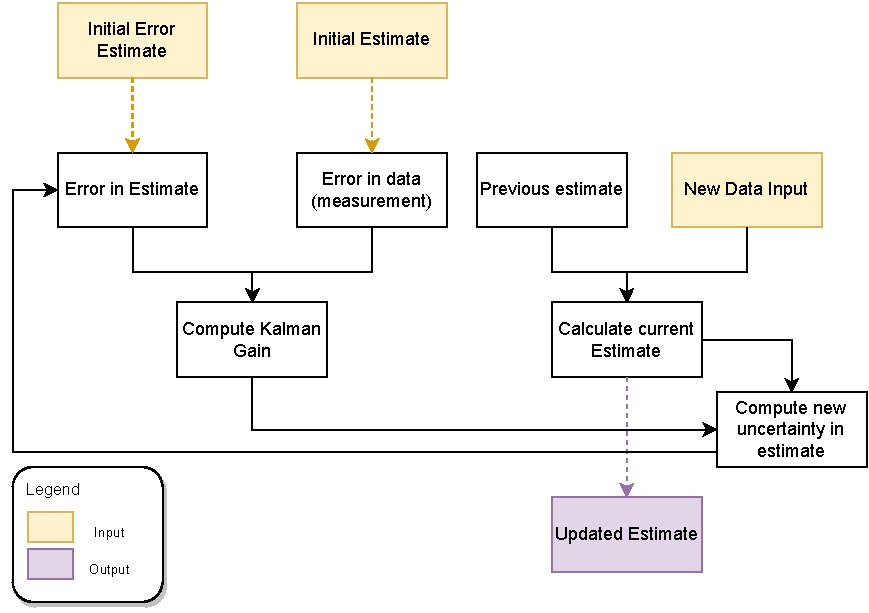
\includegraphics[width=0.6\linewidth]{images/background/Kalman-diagram.pdf}
    \caption{Simple flowchart of the Kalman Filter. \textcolor{red}{ADD REFERENCE}}
    \label{fig: flowchart kalman}
\end{figure}

In real world it is uncommon to have a global linear system and due to it's linearity, the Kalman Filter won't work well in nonlinear scenarious. A simple way to solve this is to make the global nonlinear function, locally linear, using a first order Taylor Expansion to do the aproximation. This is the approach taken by the \acl{EKF} (\acs*{EKF}) method. A more accurate way to solve the problem is to use a \acl*{UKF} (\acs*{UKF}). Instead of linearizing the original function, the \acs*{UKF} uses an Unscented Transformation\footnote{The Unscened transform picks a few points from the distribution of the input variable, then it passes them through the nonlinear function and computes the mean and standard deviation of the output. A complete explanation is given in Annex} to pass the normal distribution through the nonlinear function.

\subsection{Loop Closure}

As mentioned before, sensors used to capture information of the real world have uncertainties associated with each measurement. Even when algorithms are implemented to diminish these errors, they never vanish completely. When performing \acs*{SLAM}, a moving robot's perception and performance can be severely affected by these inaccuracies as they accumulate and become increasingly large. In the case of a pose error, in each iteration odometry information is combined with the previous pose, both of which are subject to uncertainty. Over time, the cumulative error of the robot will increase significantly. A periodic reset of the pose error would greatly improve the system. Essentially, Loop Closure achieves this goal.

\todo[inline]{Maybe talk briefly on some algorithms}

\section{Algorithms to perform \acs*{SLAM}}



\section{\acs{ROS}}

An effective robotics project cannot be achieved by just having sensors and physical components; rather, one must have a clever communication system between sensors and processes. Although such complex systems can be built from scratch, it is not worthwhile when software like \acs*{ROS} is available.

Although the name \acl*{ROS} suggests that ROS is an operating system, this is not the case.  In a way, \acs*{ROS} is both middleware and a framework. The system provides a communication channel where messages can be easily subscribed, published and distributed, allowing quick integration between systems and components. Moreover, it provides features such as debugging, visualization, testing, logging, and configuration right out of the box. Additionally, ROS includes a number of useful packages for essential areas relevant to robotics such as movement, perception, and manipulation. The ROS community is also constantly evolving with the most recent developments in robotics, so libraries are always being added to ROS. In robotics, it is considered the standard platform for developing complex projects.

\subsection{Implementation of \acs*{SLAM} algorithms in \acs*{ROS}}



\section{Related Data Acquisition Apparatus}

It is no surprise that there are already a number of portable and light sensors designed to collect sensor data about the environment around us. There are several proprietary solutions available on the market for gathering sensory information for \acs*{SLAM}, but they tend to be expensive \cite{libackpack_C50}, \cite{libackpack_DGC50}. Additionally, there are some articles and research papers that have been conducted with the goal of building a system similar to the one proposed here. These works will be the ones to be focused on since the methodology, and results are readily available.

There exist multiple ways to scan a forest, Oveland et al. \cite{oveland_comparing_2018} compared three different ground LiDAR scanning implementations, namely, Handeld LiDAR, Backpack LiDAR (composed by two \acs*{LiDAR} perpendicular to each other) and Terrestial LiDAR. The authors compared the measurements of \acs*{DBH} to conclude that while the Terrestial LiDAR Scanners (a fixed system) is the most accurate, it fails to detect ocult areas. According to the authors the handheld LiDAR scanner has troubles in detecting smaller trees. Even tho the backpack LiDAR has the highest number of false trees, the authors still aknowledge as the most efficient method since it presents the highest amount of trees detected and low values for \acs*{RMS}.

\todo[inline]{Talk about \cite{su_development_2021}}

Recently, Kui Xao developed a dual \acs*{LiDAR}s system, an \acs*{IMU}, and \acs*{GPS} for performing \acs*{SLAM} in multi-scene applications \cite{xiao_high-precision_2022}. To increase the vertical \acl*{FOV} (\acs*{FOV}), one of the \acs*{LiDAR}s was placed in the \textit{XY} plane while the other was positioned at -77.94° from the \textit{XY} plane. A timestamp synchronization algorithm is used by the authors to merge the data of the two \acs*{LiDAR}s. Secondly, the \acs*{LiDAR} data is tightly coupled with the IMU data in order to reduce noise caused by the inaccuracy of \acs*{LiDAR}-based odometry. In outdoor tests, the \acs*{IMU} calibration is improved by loosely coupling \acs*{GPS} to the \acs*{IMU} during outdoor tests.

In terms of application, Alexander Proudman's system is closest to this project's \cite{proudman_online_2021}. Based on an Ouster OS0-128 \acs{LiDAR} and a RealSense D435i, both with an integrated \acs{IMU}, the system performs online \acs{SLAM} and estimates \acl{DBH} (\acs*{DBH}) using the data collected. While their application has the benefit of having a built-in display that allows real-time visualization of data, one of its major drawbacks is the way they build their apparatus, opting for a metal stick rather than a backpack type of design. As the authors acknowledge, user fatigue may lead to excessive variations in stick position, resulting in unintelligible and uncontrolled movements, damaging the performance of the apparatus.This would not be an issue if a more ergonomic structure was used. The errors due to user fatigue can be a slightly mitigated by performing \acs{SLAM} in several sessions instead of one, allowing the user to rest between shorter sessions \textcolor{red}{INSERT REFERENCE TO THE SECOND PAPER}. After recording multiple sessions, \acs*{GPS} information is used to assemble the multiple sessions's map into a single map.